\chapter{案例研究}
\section{Solid Edge 應用範例}
圖\ref{3.20}為利用Solid Edge所設計的機器人,如今,Solid Edge 2023 透過同步建模簡化了許多設計工作流程,因此可以在使用 CAD 軟件的日常工作中以更少的點擊次數更快地實現目標。\\
\begin{figure}[hbt!]
\begin{center}
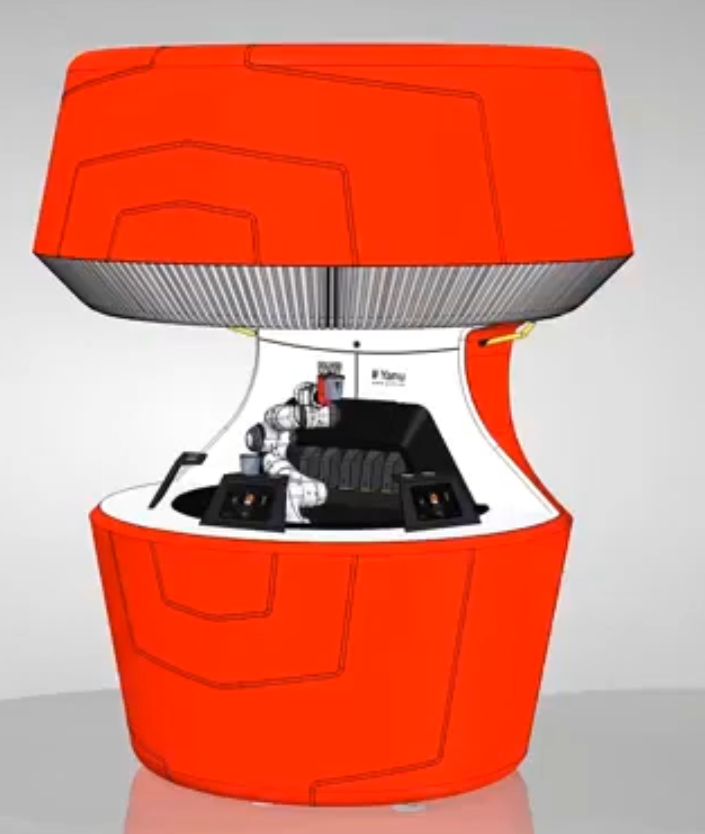
\includegraphics[width=10cm]{se8}
\caption{\Large Solid Edge 機器人}\label{3.20}
\end{center}
\end{figure}
\\
\begin{figure}[hbt!]
\begin{center}
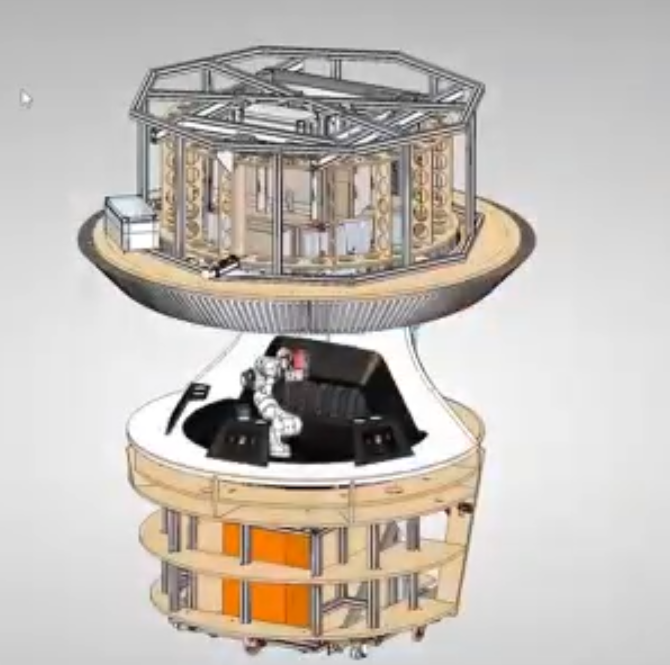
\includegraphics[width=8cm]{se5}
\caption{\Large Solid Edge 機器人}\label{3.27}
\end{center}
\end{figure}
\\
我們在需要建模的草圖上(圖\ref{3.21}),只需要透過滑鼠的移動就能很快的建立外型,只要點選需要的面向上(拉伸)或向下(除料)拖移即可建立特徵,如圖\ref{3.22}(拉伸 )與圖\ref{3.23}(除料)所示。\\
\begin{figure}[hbt!]
\begin{center}
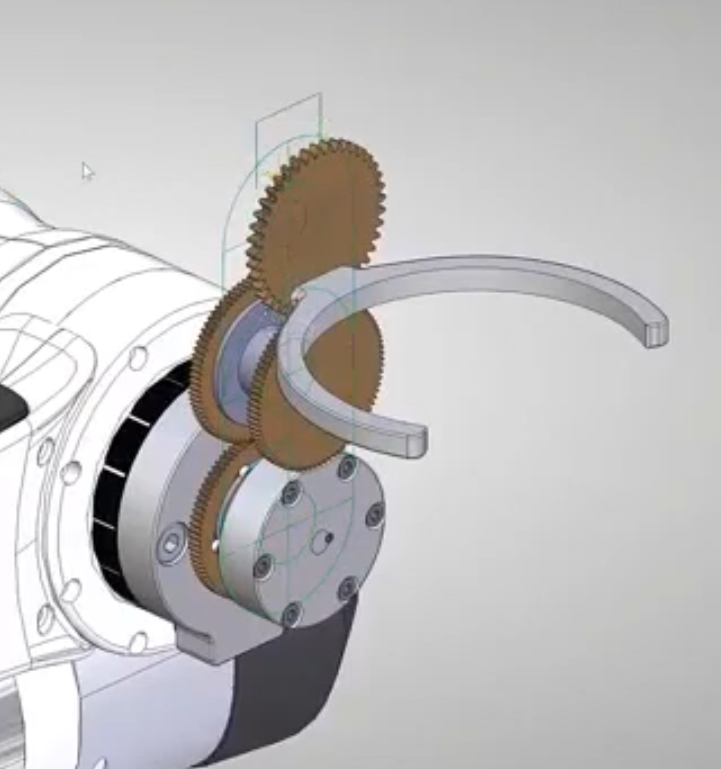
\includegraphics[width=8cm]{se1}
\caption{\Large Solid Edge建模}\label{3.21}
\end{center}
\end{figure}
\\
\begin{figure}[hbt!]
\begin{center}
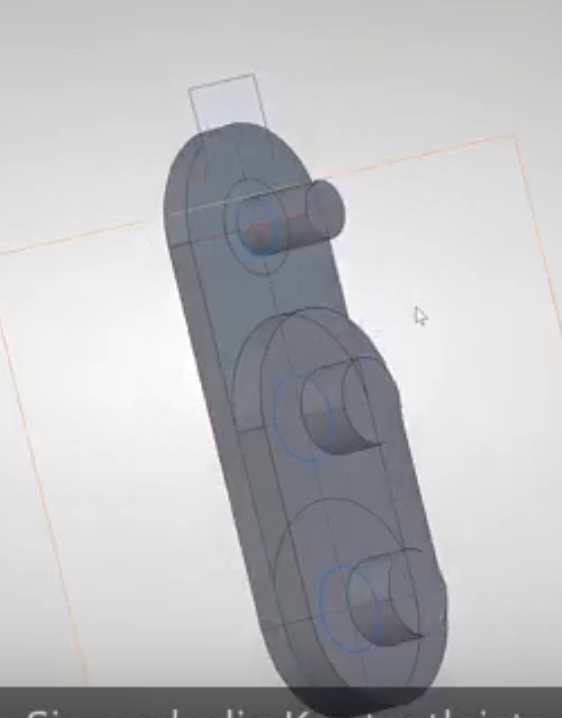
\includegraphics[width=8cm]{se7}
\caption{\Large Solid Edge拉伸}\label{3.22}
\end{center}
\end{figure}
\\
\begin{figure}[hbt!]
\begin{center}
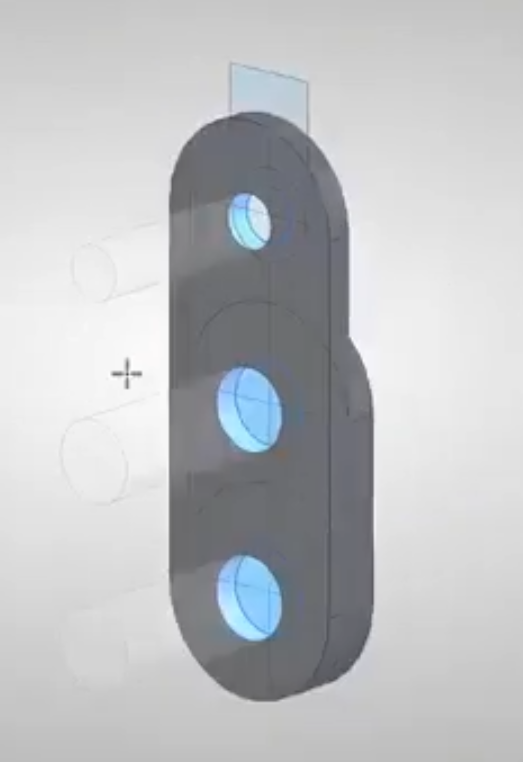
\includegraphics[width=8cm]{se3}
\caption{\Large Solid Edge除料}\label{3.23}
\end{center}
\end{figure}
\\
建完模後,不需再調整其他模型,因為同步建模的關係,會自動移動其他零件,不需要害怕會干擾到其他零件或特徵,減少了需要再設定特徵或約束關係的時間(圖\ref{3.24});零件上色也非常方便且迅速,透過滑鼠拖移的動作即可完成(圖\ref{3.25})。\\
\begin{figure}[hbt!]
\begin{center}
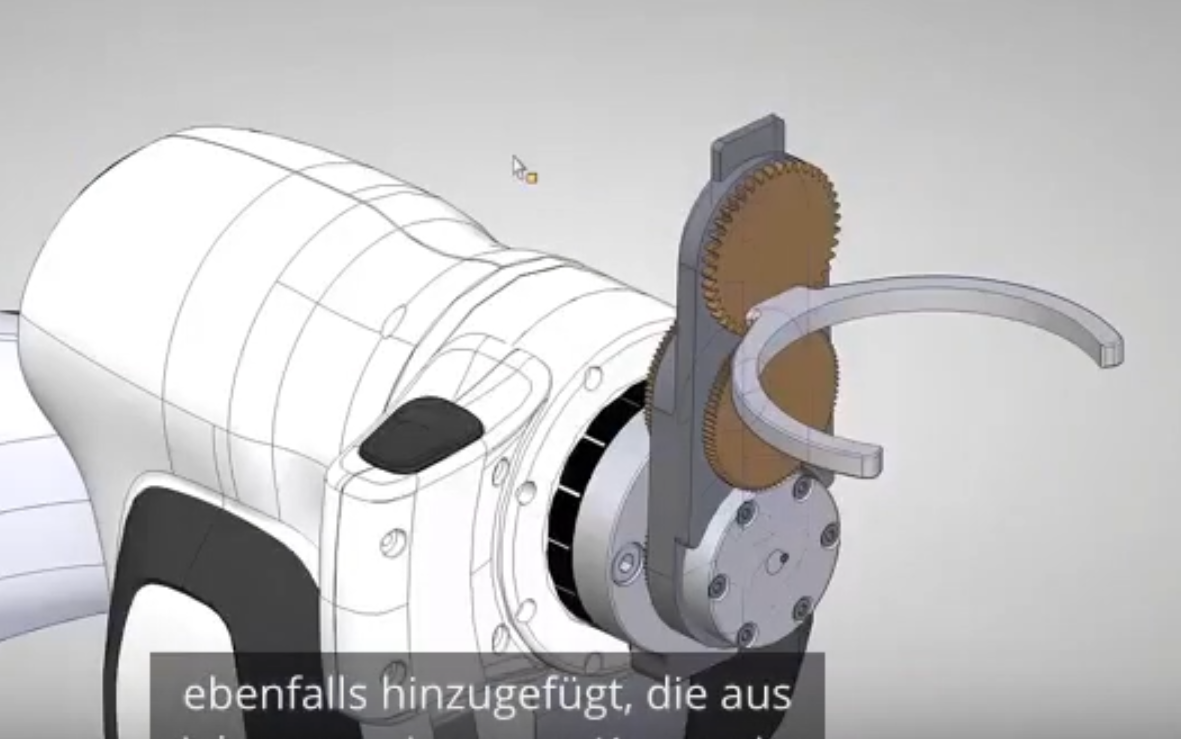
\includegraphics[width=10cm]{se6}
\caption{\Large Solid Edge建模完成}\label{3.24}
\end{center}
\end{figure}
\\
\begin{figure}[hbt!]
\begin{center}
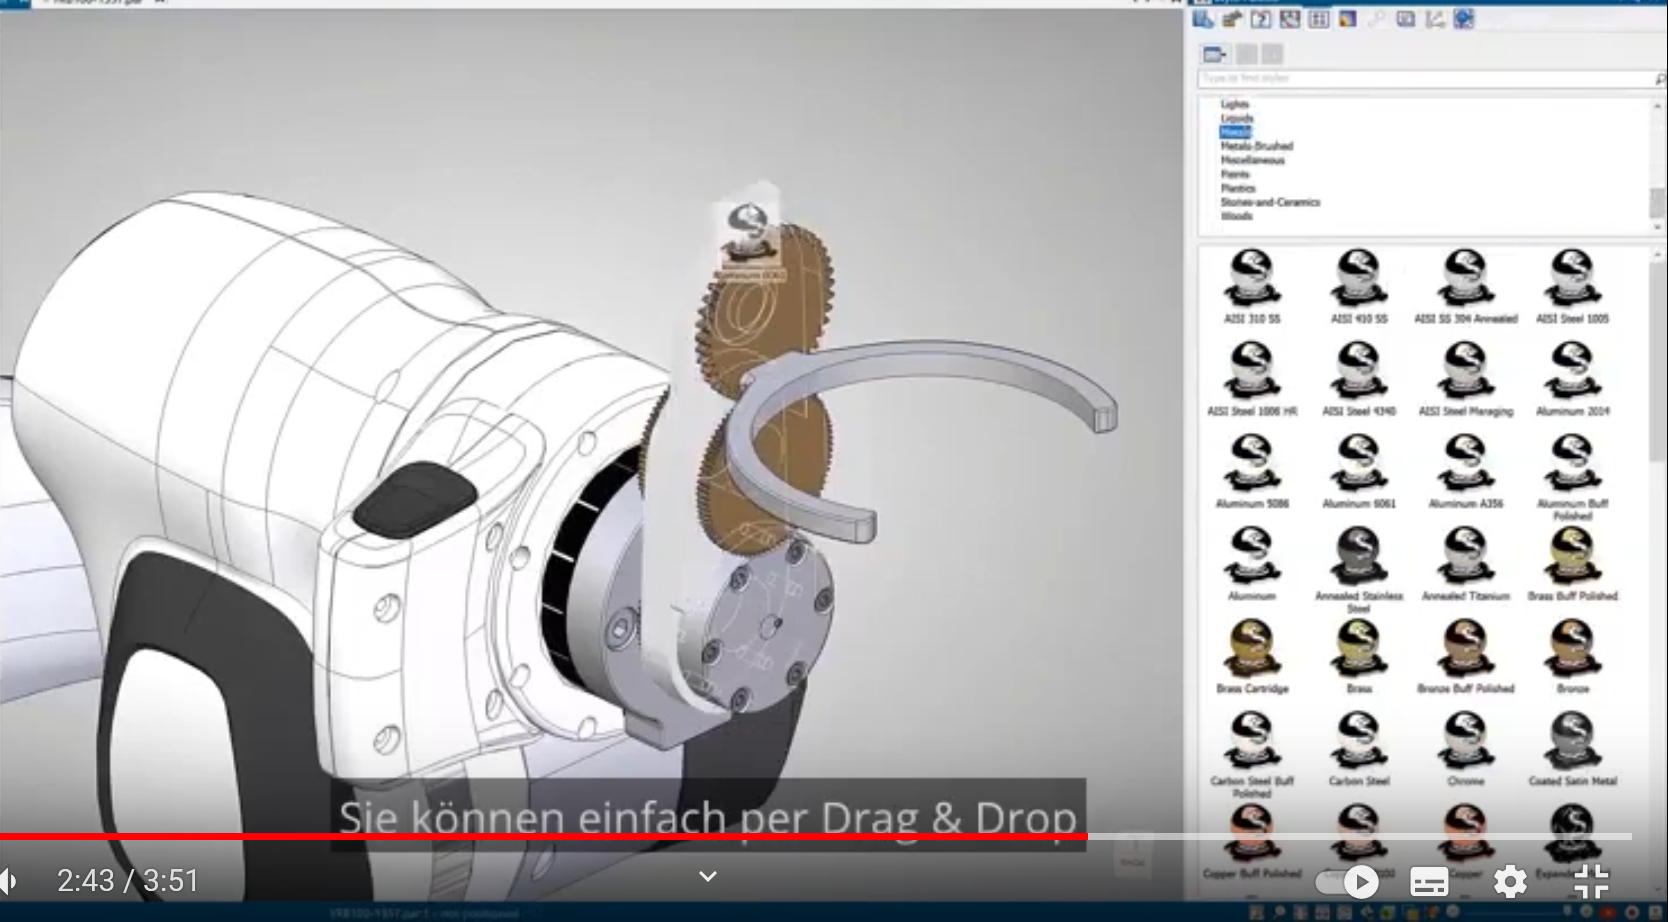
\includegraphics[width=10cm]{se4}
\caption{\Large Solid Edge零件上色}\label{3.25}
\end{center}
\end{figure}
\\
在 Solid Edge 2023 中,Extras > “Visual explode”選項卡中有新命令用於裝配體的分解視圖。這些可以幫助您在現場快速了解裝配體的結構,而無需事先創建和保存耗時的爆炸。您可以使用簡單的滑塊分解裝配體,或智能地逐步分解子裝配體。(圖\ref{3.26})\\
\begin{figure}[hbt!]
\begin{center}
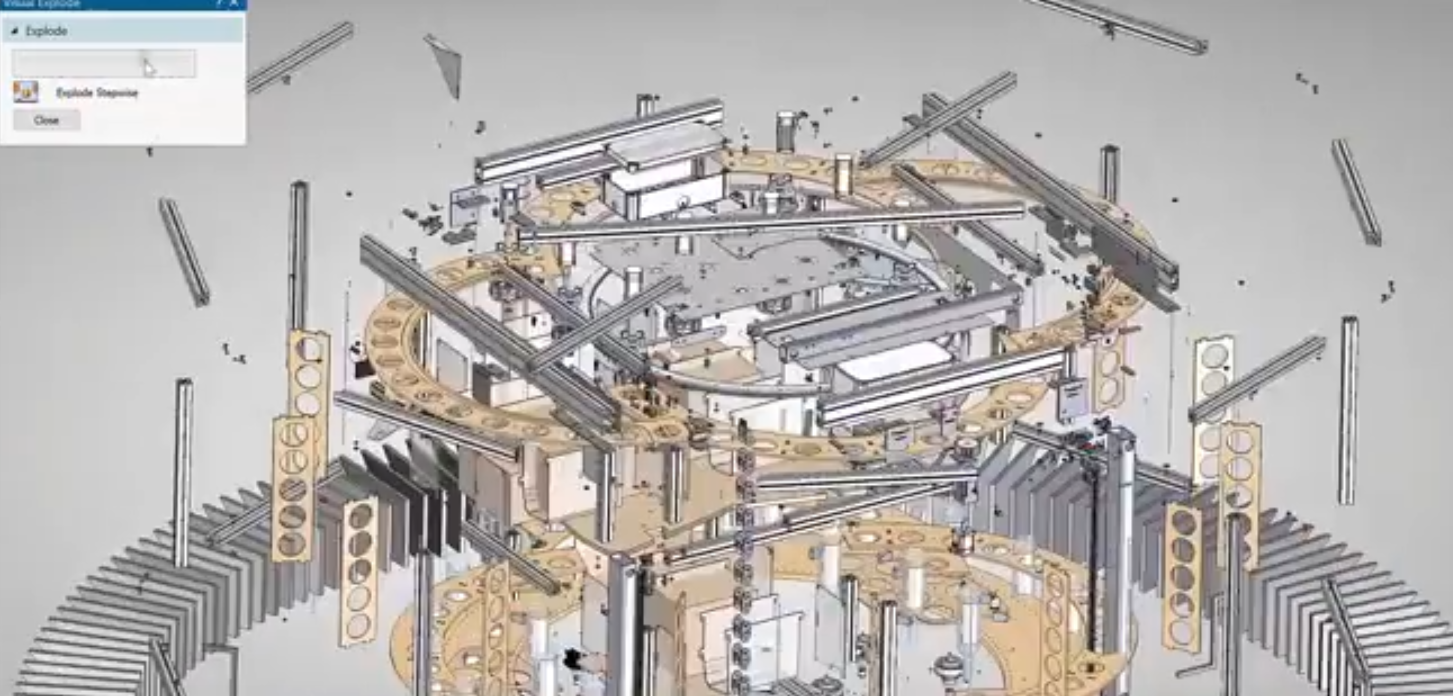
\includegraphics[width=14cm]{se9}
\caption{\Large Solid Edge分解視圖}\label{3.26}
\end{center}
\end{figure}
\\

\newpage

\section{Femap應用範例}
\begin{itemize}
\item 過程模擬(圖\ref{3.02})\\
\begin{figure}[hbt!]
\begin{center}
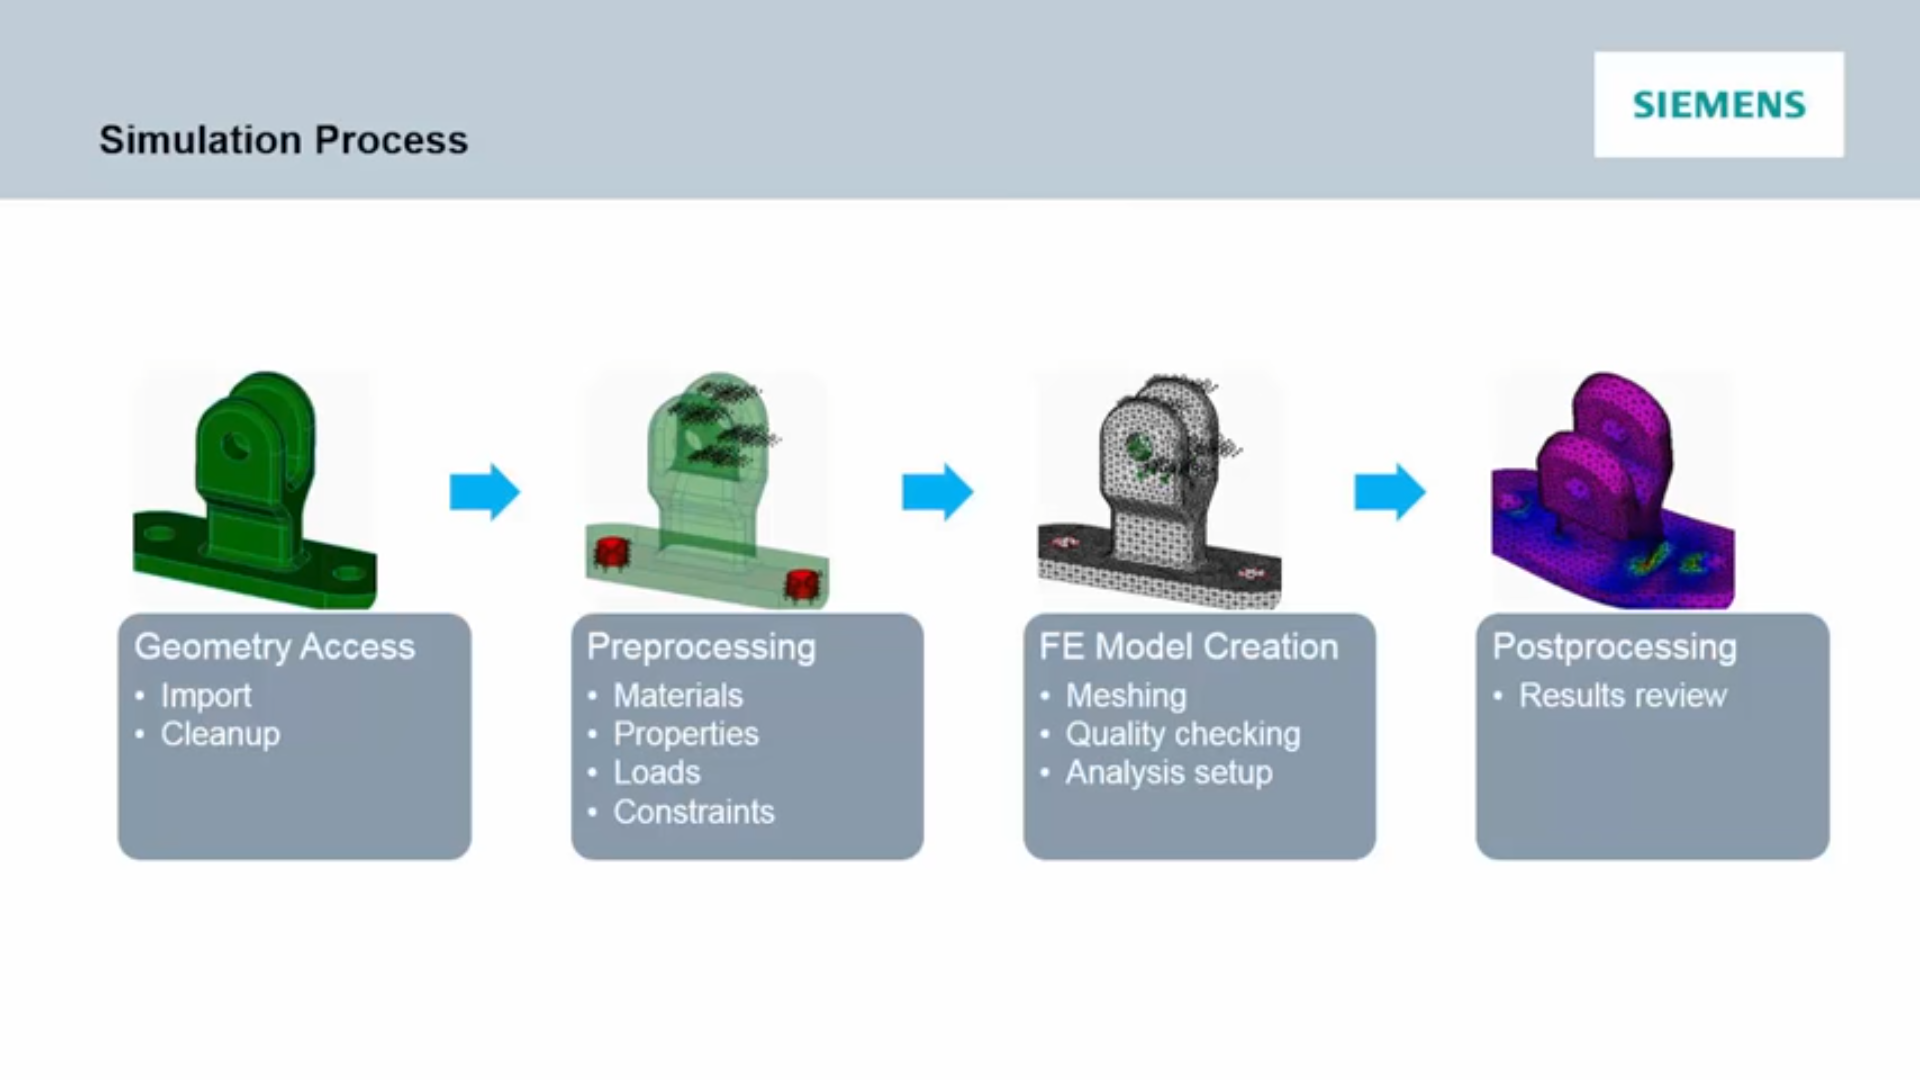
\includegraphics[width=14cm]{Femap1}
\caption{\Large 模擬過程}\label{3.02}
\end{center}
\end{figure}
\\
\qquad 由上圖可知Femap的簡約分析設定過程,大致上能分成四大步驟:\\

1.幾何導入和準備\\
\qquad 將建立好的模型輸入到Femap裡,進行清理的動作,讓下一階段的預處理方便執行。\\
\qquad Femap可以不須轉檔,就能直接讀取SolidWorks、Solid Edge、Autodesk...等知名繪圖軟體的繪圖檔,也能透過STEP、IGES、DXF...等檔案輸入進行分析。\\
\begin{figure}[hbt!]
\begin{center}
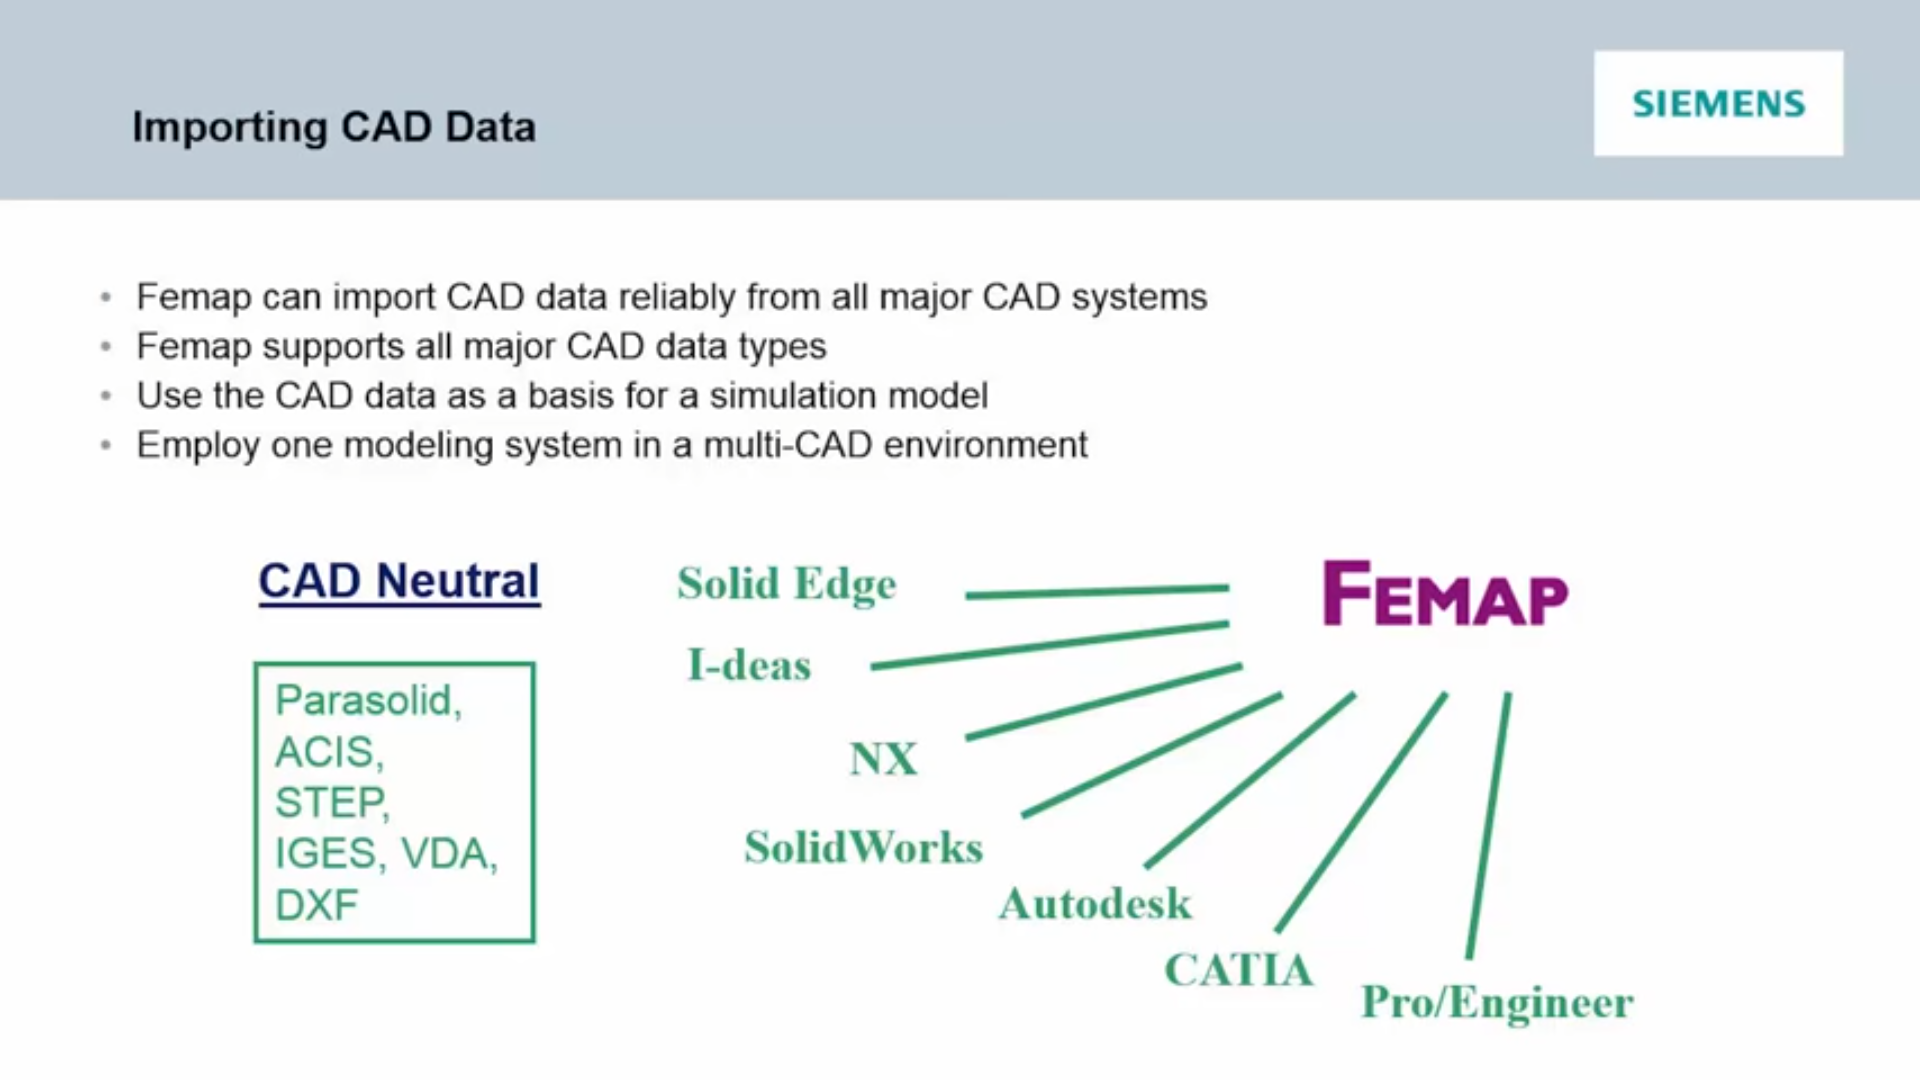
\includegraphics[width=12cm]{Femap2}
\caption{\Large Femap Simulation Process}\label{3.03}
\end{center}
\end{figure}
\\
\qquad 以機械手臂的零組件為例,完成模型幾何的輸入後,使用各種清理命令清理幾何圖形,以便為進一步的後處理做好先前準備。\\

\qquad 由圖\ref{3.01}為例,能用Geomotry的Cleanup指令來清理模型上的線架構,將一段分成多段的線直接合併成一段,讓進一步的網格化個好處理。\\
\begin{figure}[hbt!]
\begin{center}
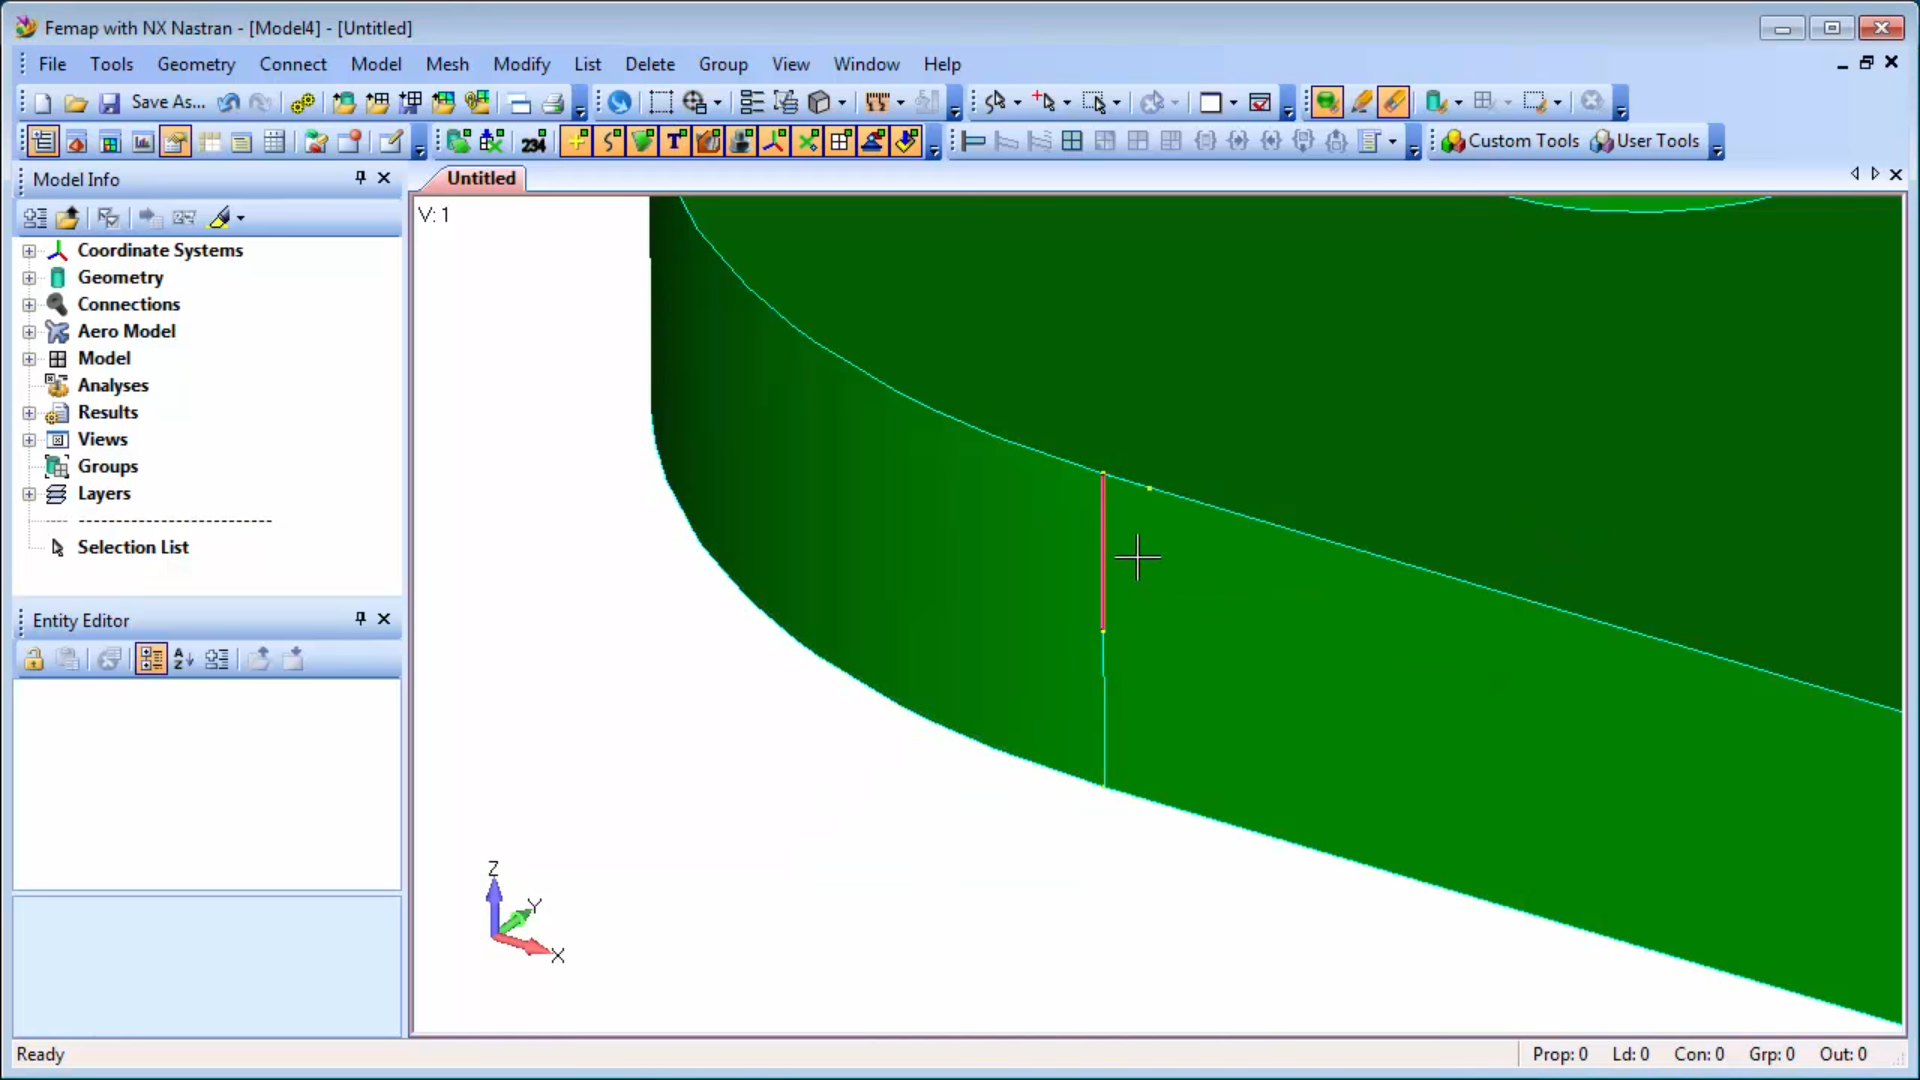
\includegraphics[width=14cm]{Femap3}
\caption{\Large Femap Cleanup}\label{3.01}
\end{center}
\end{figure}
\\
2.預處理屬性和邊界條件\\
\qquad 材料及屬性的設定,完成後就能進行力與約束的設置。\\

\qquad 材料的輸入能在左側Model下的Materials進行設定,對其左鍵增加新的材料選擇,在圖\ref{3.04}中能看到材料的多樣性,有用不完的材料能夠分析。\\
\qquad 完成後,在Properties裡新增模型的屬性,將新增好的材料加入到其中,讓模型屬性裡頭使用所選的材料。\\
\begin{figure}[hbt!]
\begin{center}
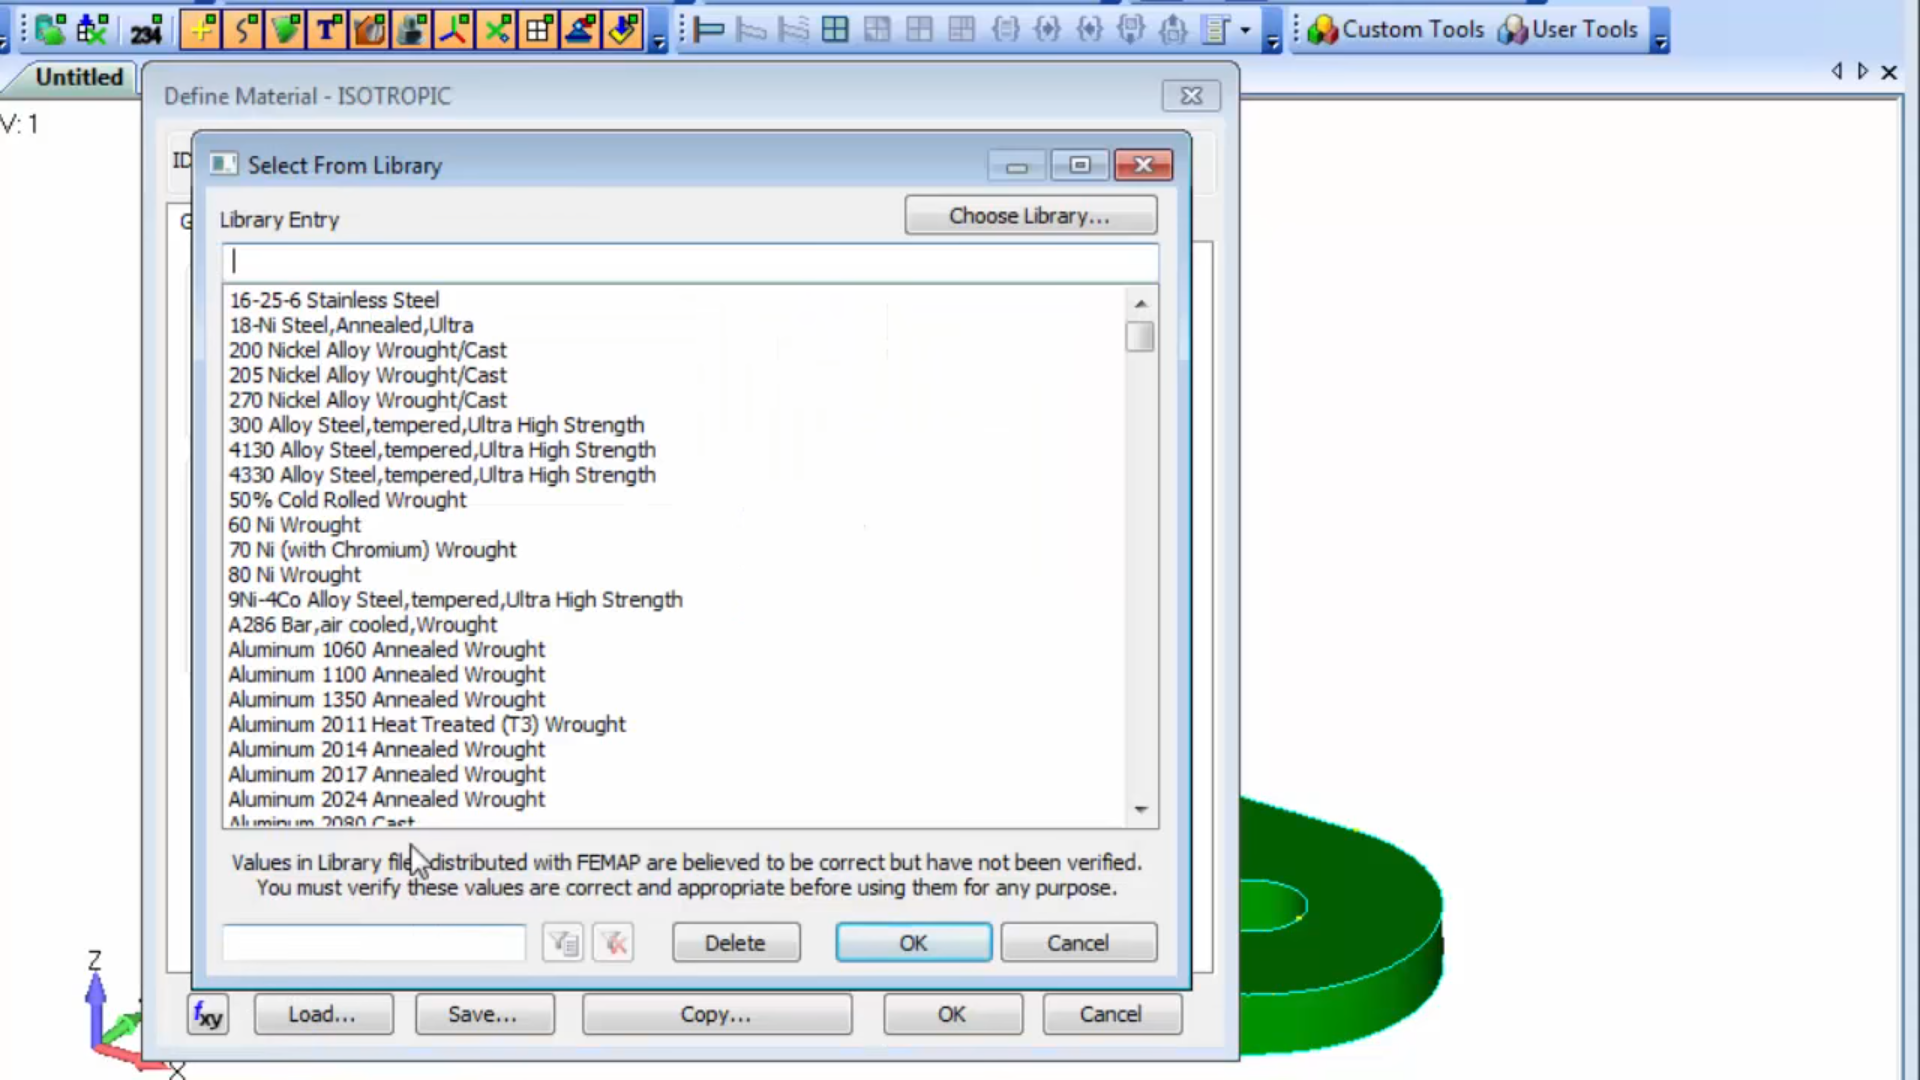
\includegraphics[width=12cm]{Femap4}
\caption{\Large Femap材料選擇}\label{3.04}
\end{center}
\end{figure}
\\
\begin{figure}[hbt!]
\begin{center}
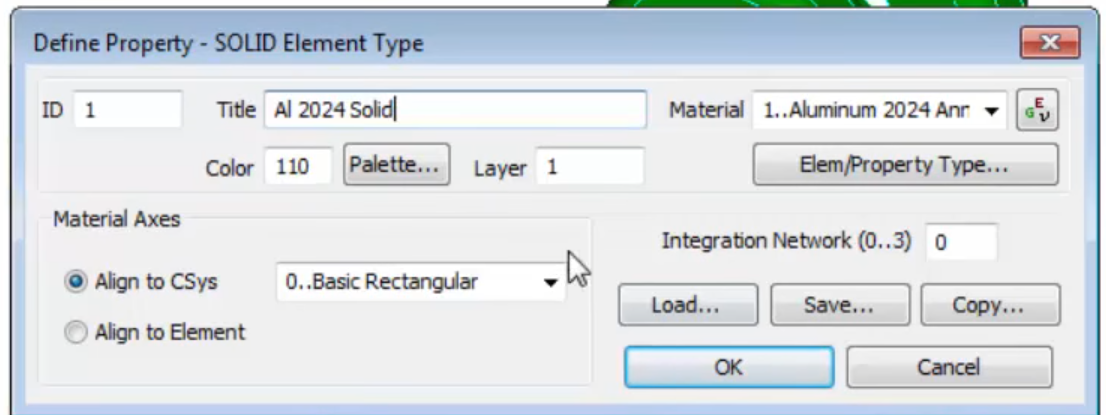
\includegraphics[width=10cm]{Femap8}
\caption{\Large Femap材料選擇}\label{3.05}
\end{center}
\end{figure}
\\
\qquad 接下來設置作用力與約束條件,Loads裡新增一個力量,在設定裡面,除了力的大小、範圍及位置外,也能調整力的角度,來滿足斜於受立面的力量設定。(圖\ref{3.05}~圖\ref{3.07})\\
\qquad 而約束條件與作用力設定模式差不多,同樣是左側Constraints新增約束項目,然後進行範圍及模式的設定。(圖\ref{3.08}、圖\ref{3.09})\\
\begin{figure}[hbt!]
\begin{center}
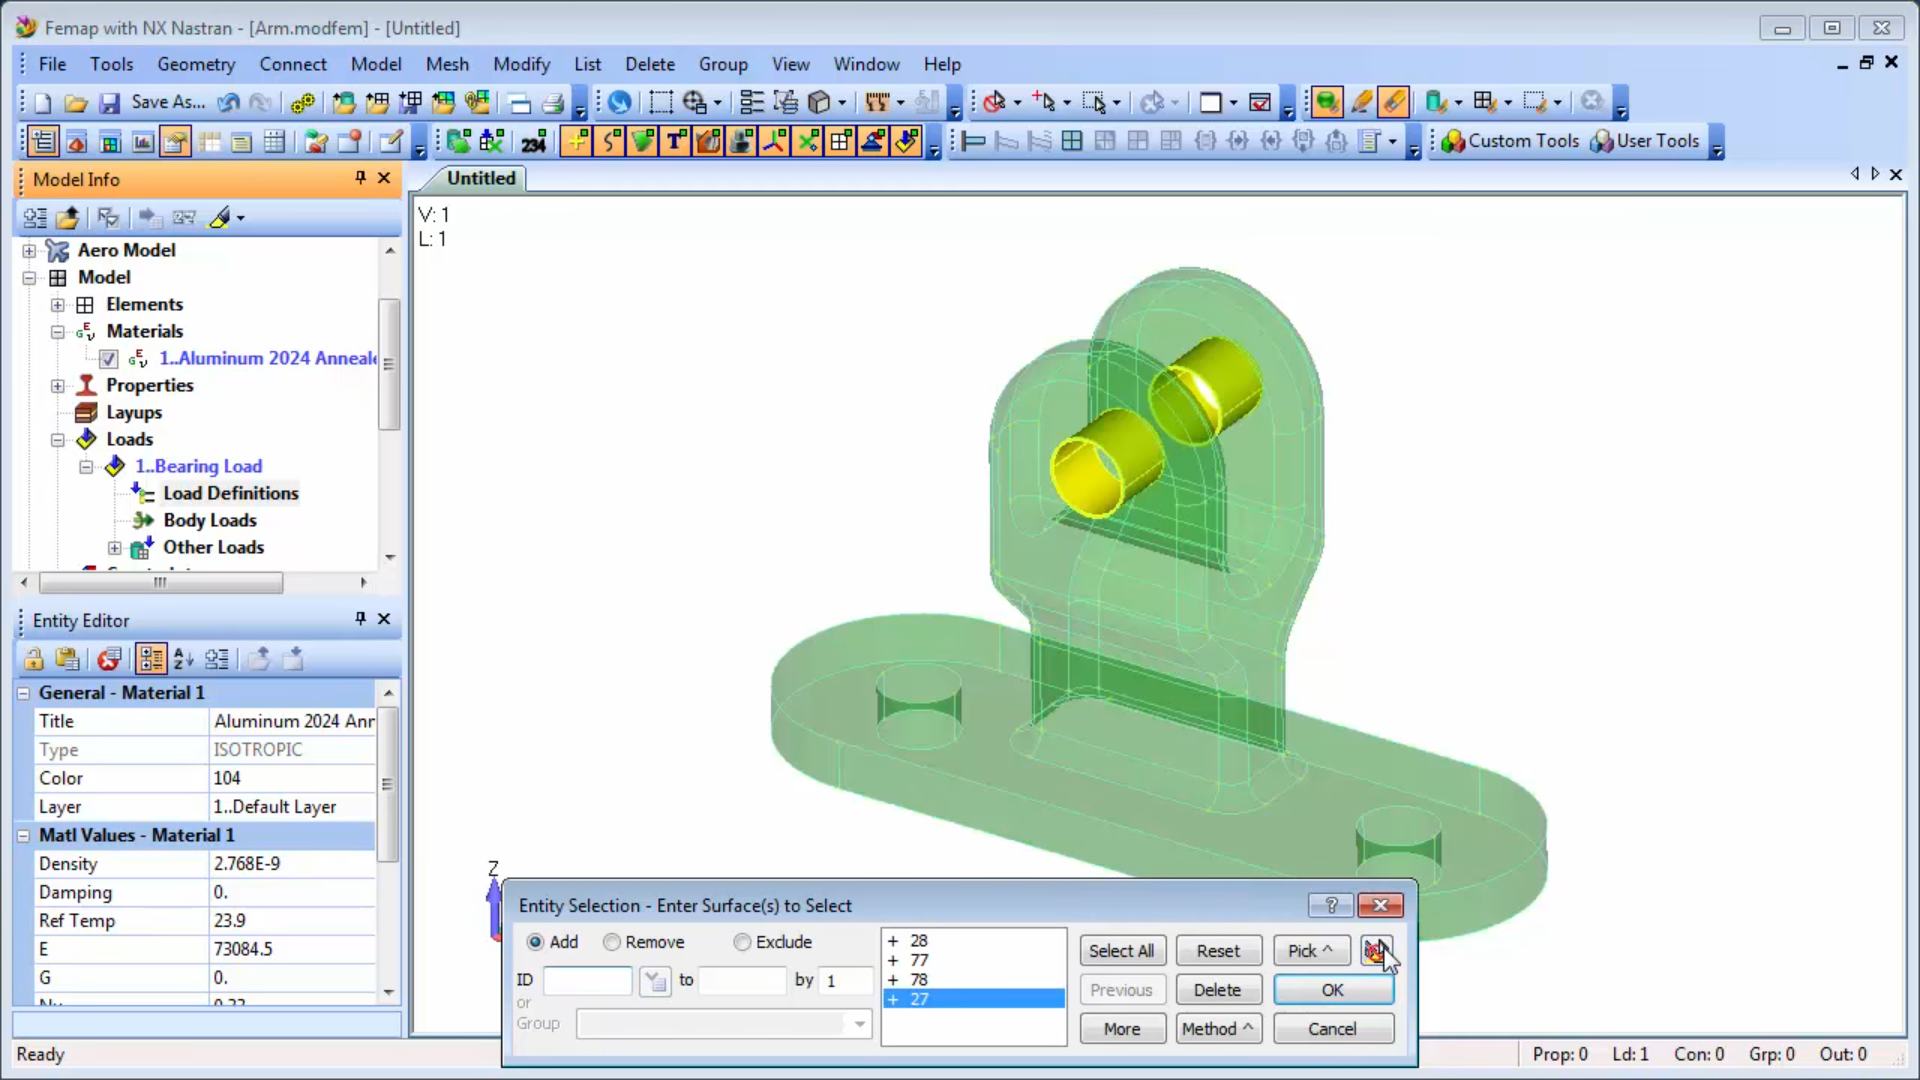
\includegraphics[width=12cm]{Femap5}
\caption{\Large Femap作用力設定}\label{3.05}
\end{center}
\end{figure}
\\
\begin{figure}[hbt!]
\begin{center}
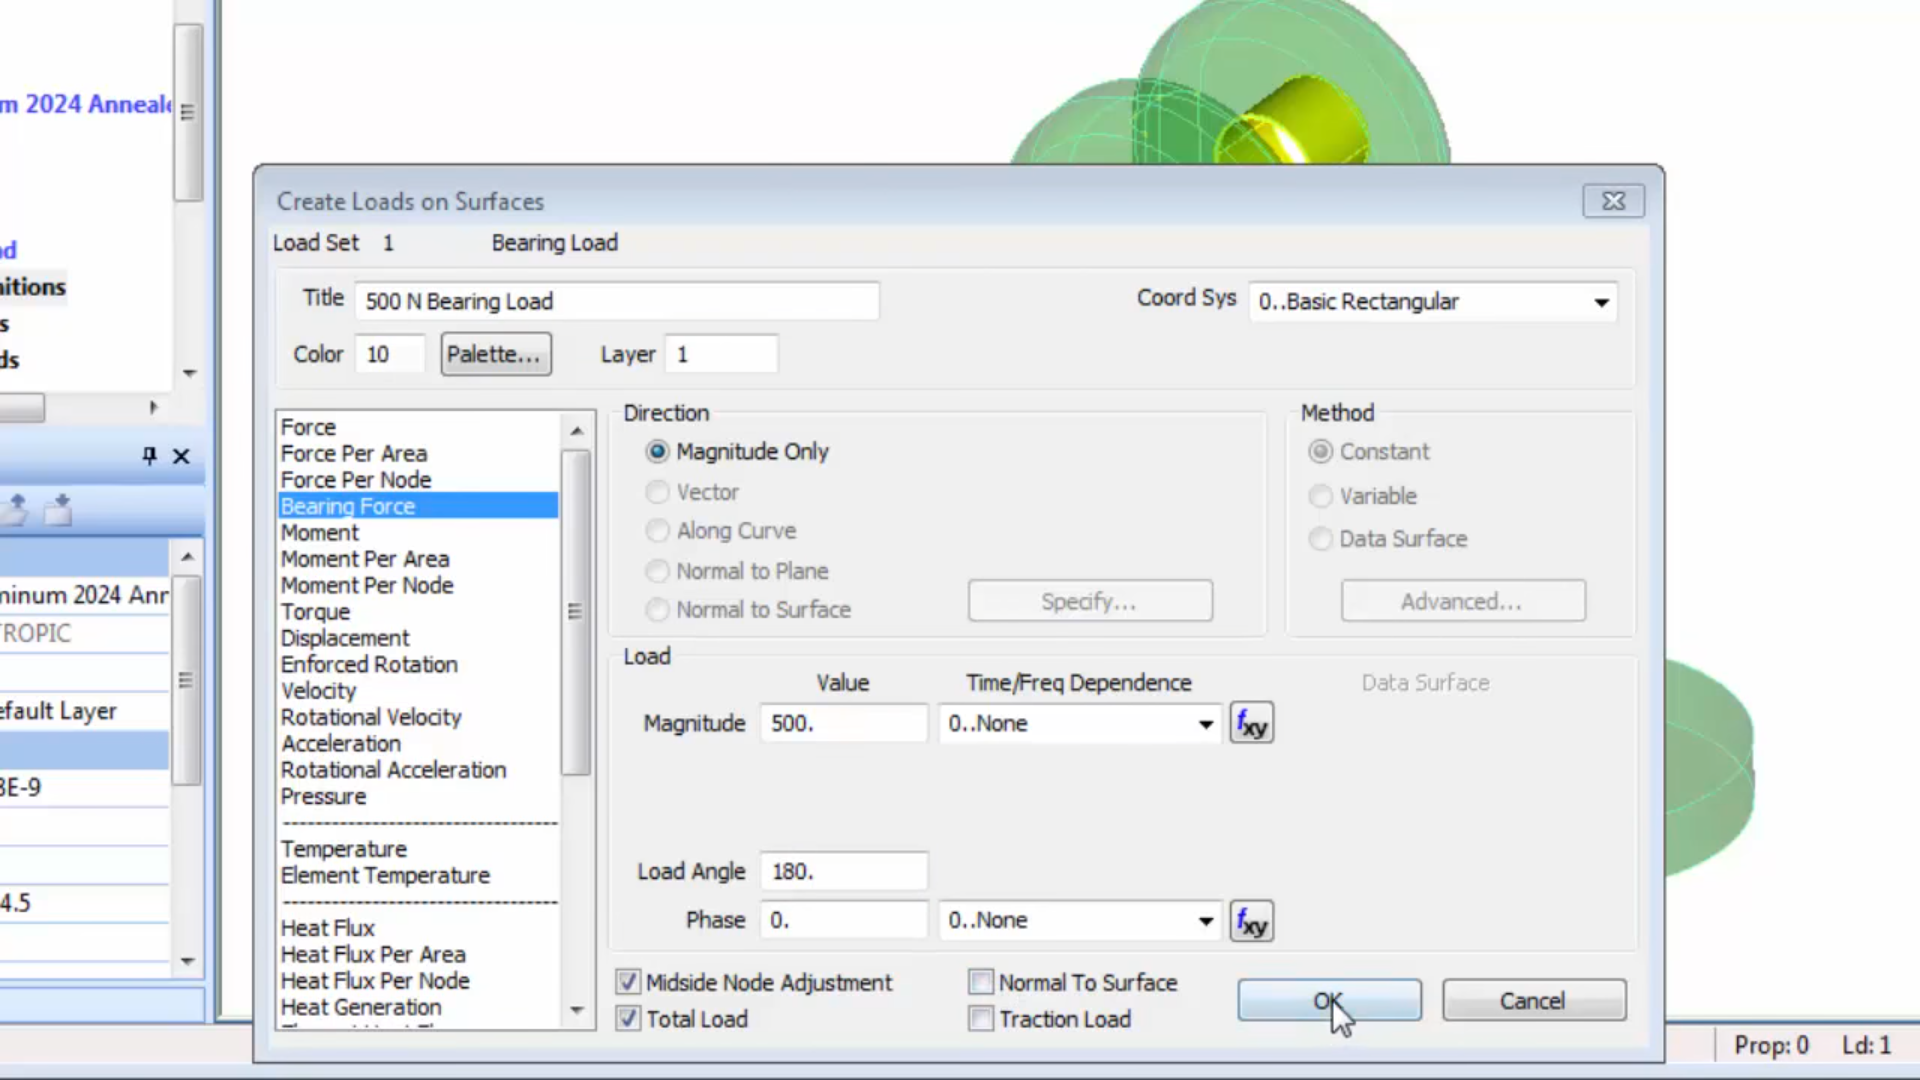
\includegraphics[width=12cm]{Femap6}
\caption{\Large Femap作用力設定}\label{3.06}
\end{center}
\end{figure}
\\
\begin{figure}[hbt!]
\begin{center}
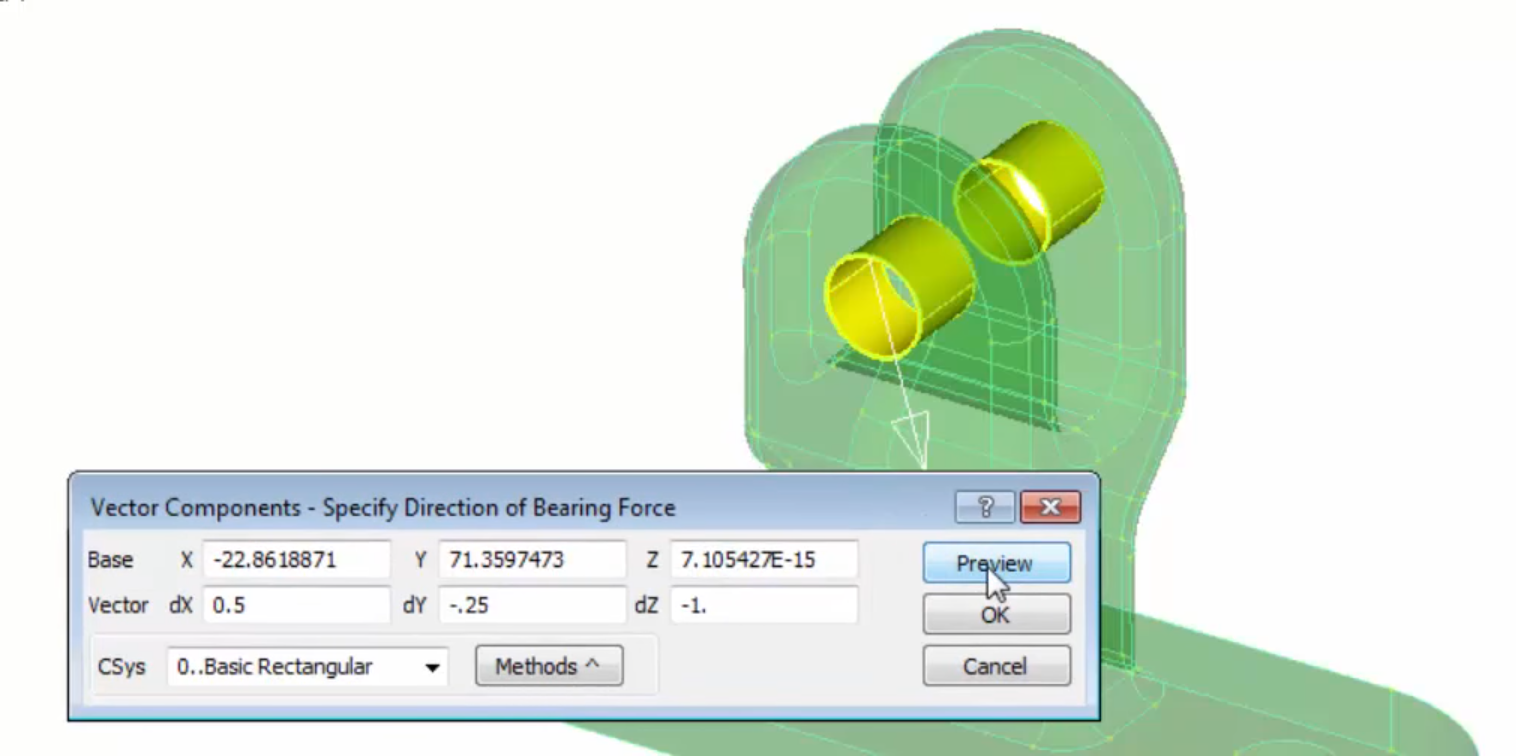
\includegraphics[width=12cm]{Femap7}
\caption{\Large Femap作用力設定}\label{3.07}
\end{center}
\end{figure}
\\
\begin{figure}[hbt!]
\begin{center}
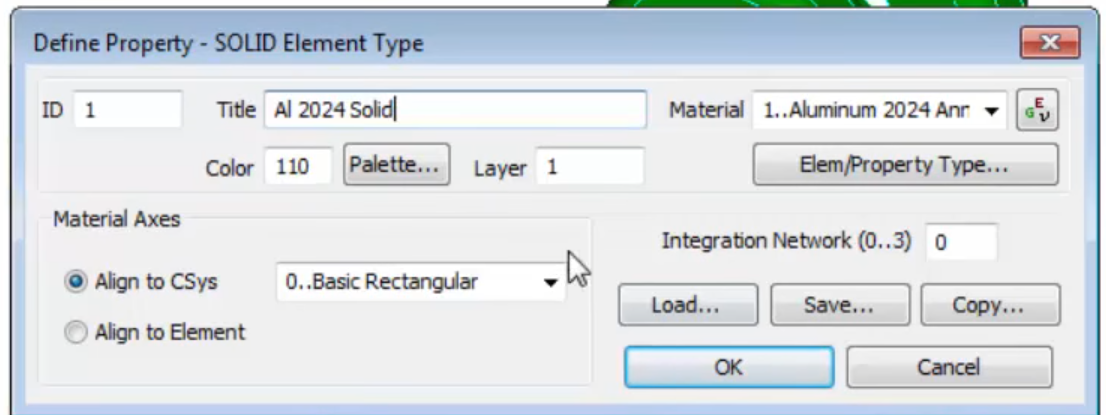
\includegraphics[width=12cm]{Femap8}
\caption{\Large Femap約束條件設定}\label{3.08}
\end{center}
\end{figure}
\\
\begin{figure}[hbt!]
\begin{center}
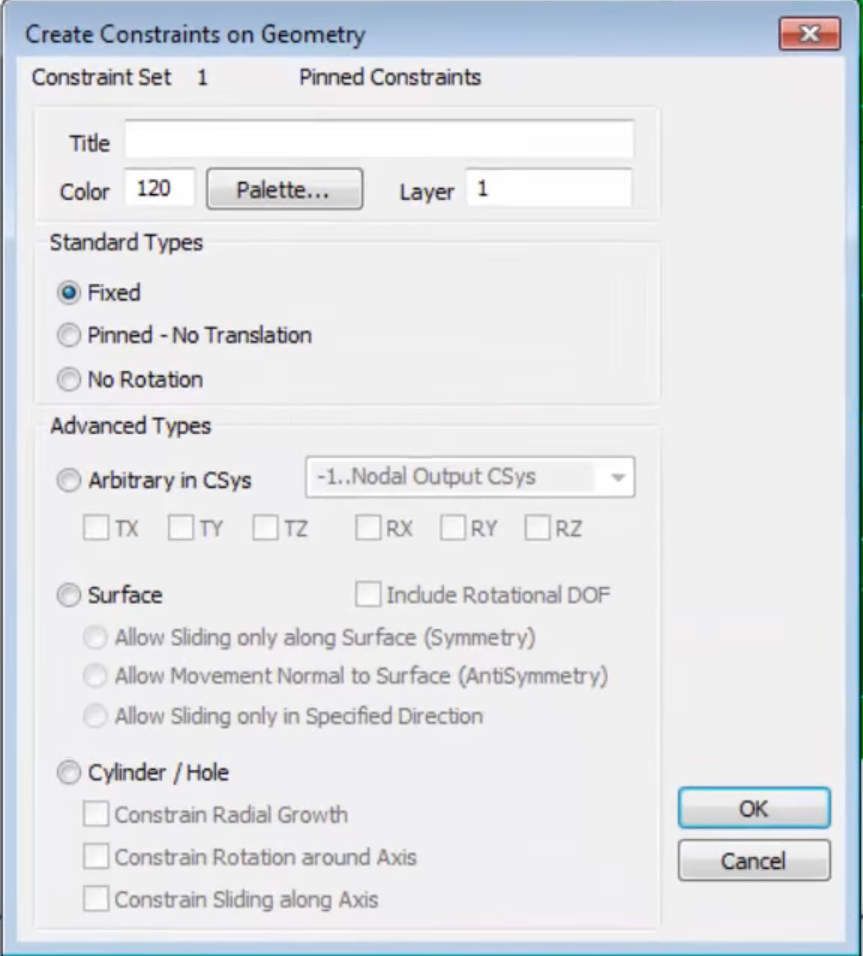
\includegraphics[width=10cm]{Femap9}
\caption{\Large Femap約束條件設定}\label{3.09}
\end{center}
\end{figure}
\\
3. 網格劃分和分析設置\\
\qquad 對幾何體進行網格劃分以創建有限元模型。然後將使用Femap分析集管理器設置分析參數。現在可以將模型提交給 NX Nastran 求解器。\\

\qquad 左側Geometry>模型>Tet Mesh裡,可以對Element Size即跟Mesh sizing相關的其他係數進行更改,這對網格化後的網格大小有關。\\
\begin{figure}[hbt!]
\begin{center}
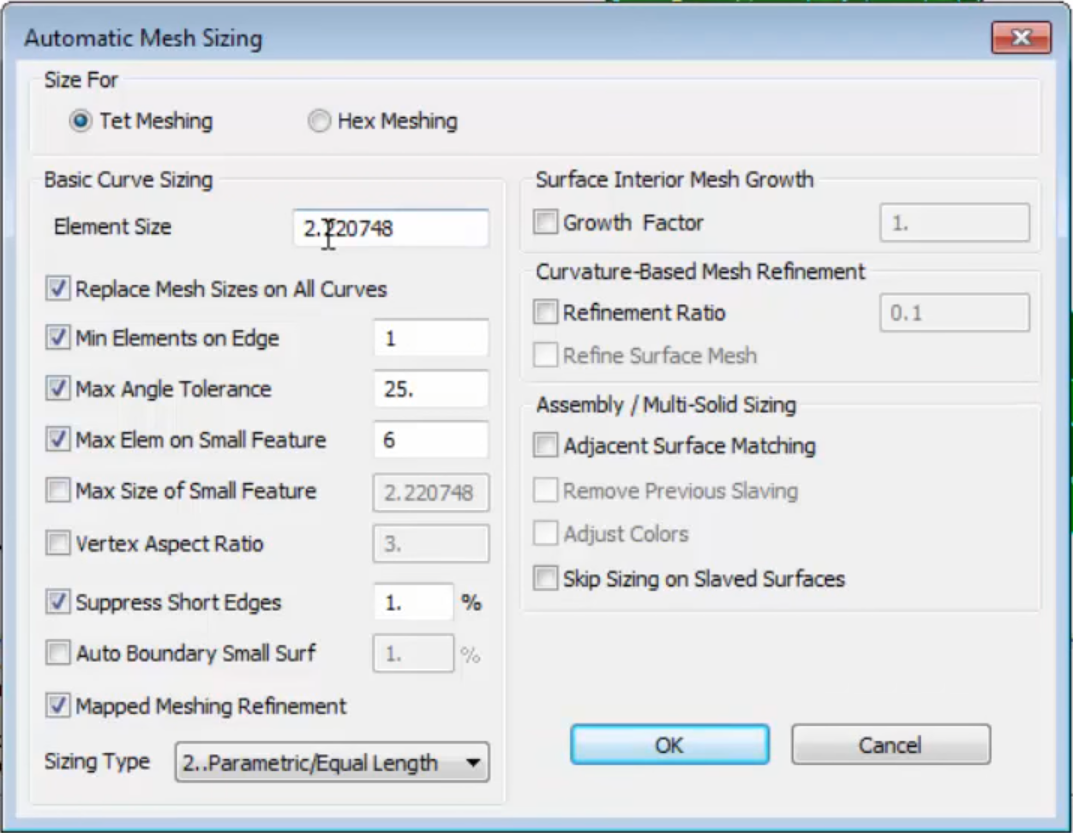
\includegraphics[width=10cm]{Femap10}
\caption{\Large Femap Mash Sizing}\label{3.10}
\end{center}
\end{figure}
\\
\qquad 接下來進行分析設置,Analyses>Manage新增想要分析的類型(圖\ref{3.11}),並確認設定的作用力及約束條件是否加入到分析內容中(圖\ref{3.12}),檢查完後按下分析後,Femap就會對你所設的條件來對模型做分析。\\
\begin{figure}[hbt!]
\begin{center}
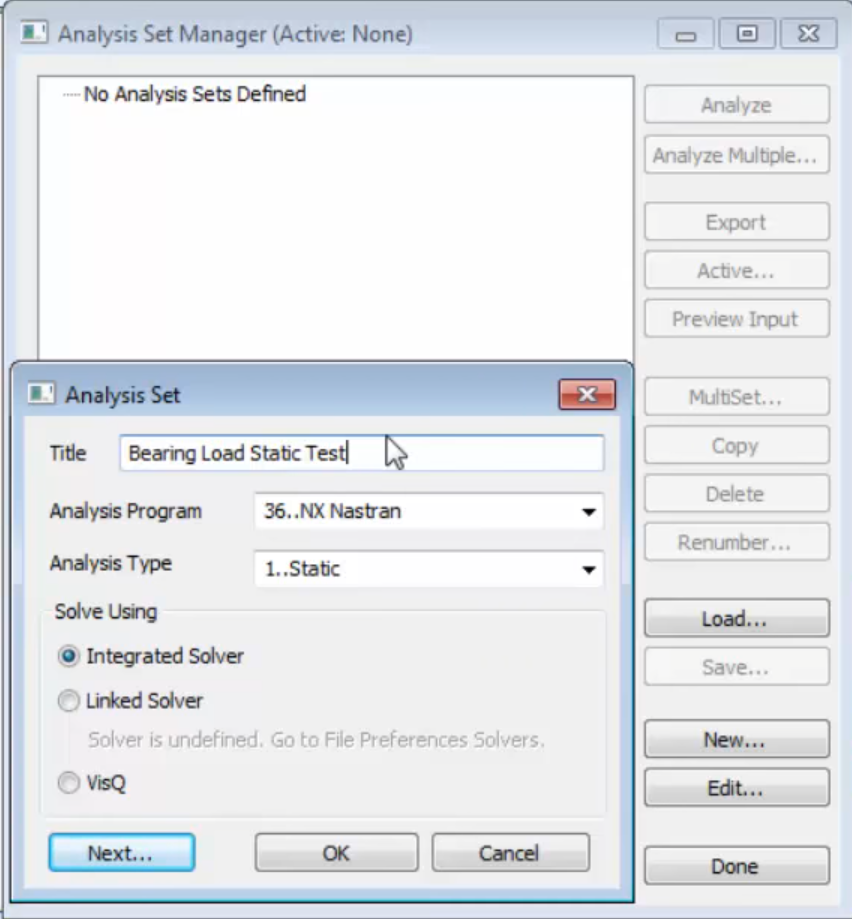
\includegraphics[width=10cm]{Femap11}
\caption{\Large Femap Analysis Set}\label{3.11}
\end{center}
\end{figure}
\\
\begin{figure}[hbt!]
\begin{center}
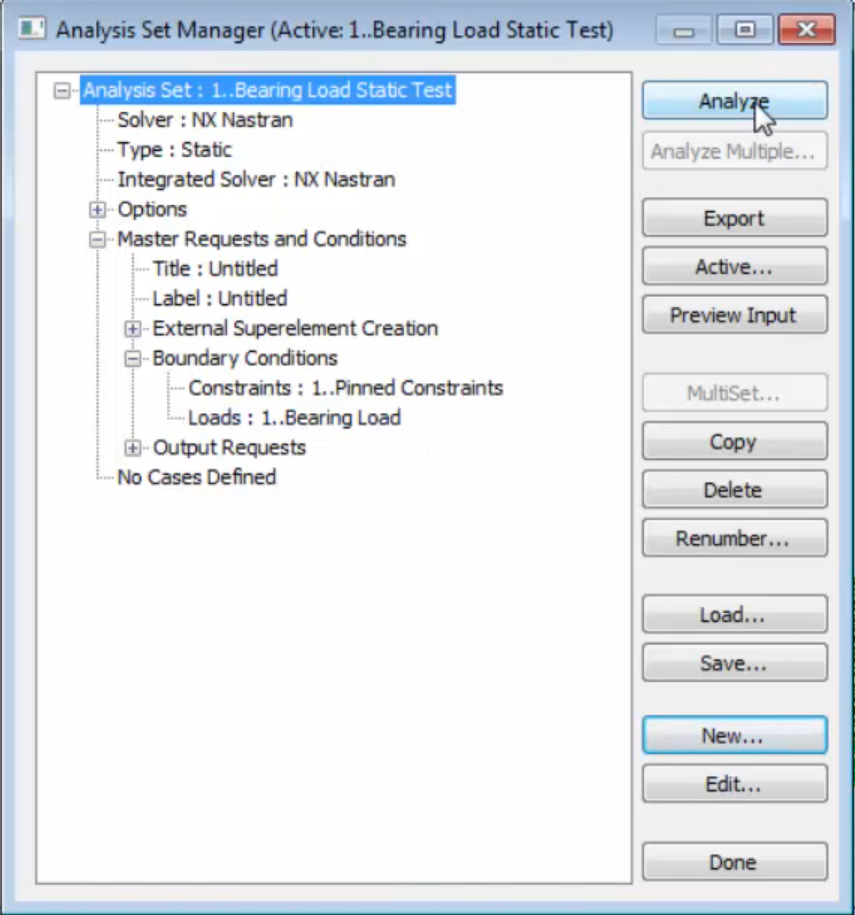
\includegraphics[width=10cm]{Femap12}
\caption{\Large Femap Analysis Set}\label{3.12}
\end{center}
\end{figure}
\\
4.後處理和結果審查\\
\qquad 查看NX Nastran計算的結果以及使用後處理工具箱在Femap中對數據進行後處理。\\

\qquad 先在圖\ref{3.13}所標示的紅色位置叫出PostProcessing Toolbox,選擇想要觀看的分析結果,如果覺得變化不大,不易觀察的話,也能在此頁面中增加變化的倍率(圖\ref{3.14}),還能有變化的動畫能觀看,讓我們能更直覺地觀察變化量(圖\ref{3.15})。\\
\begin{figure}[hbt!]
\begin{center}
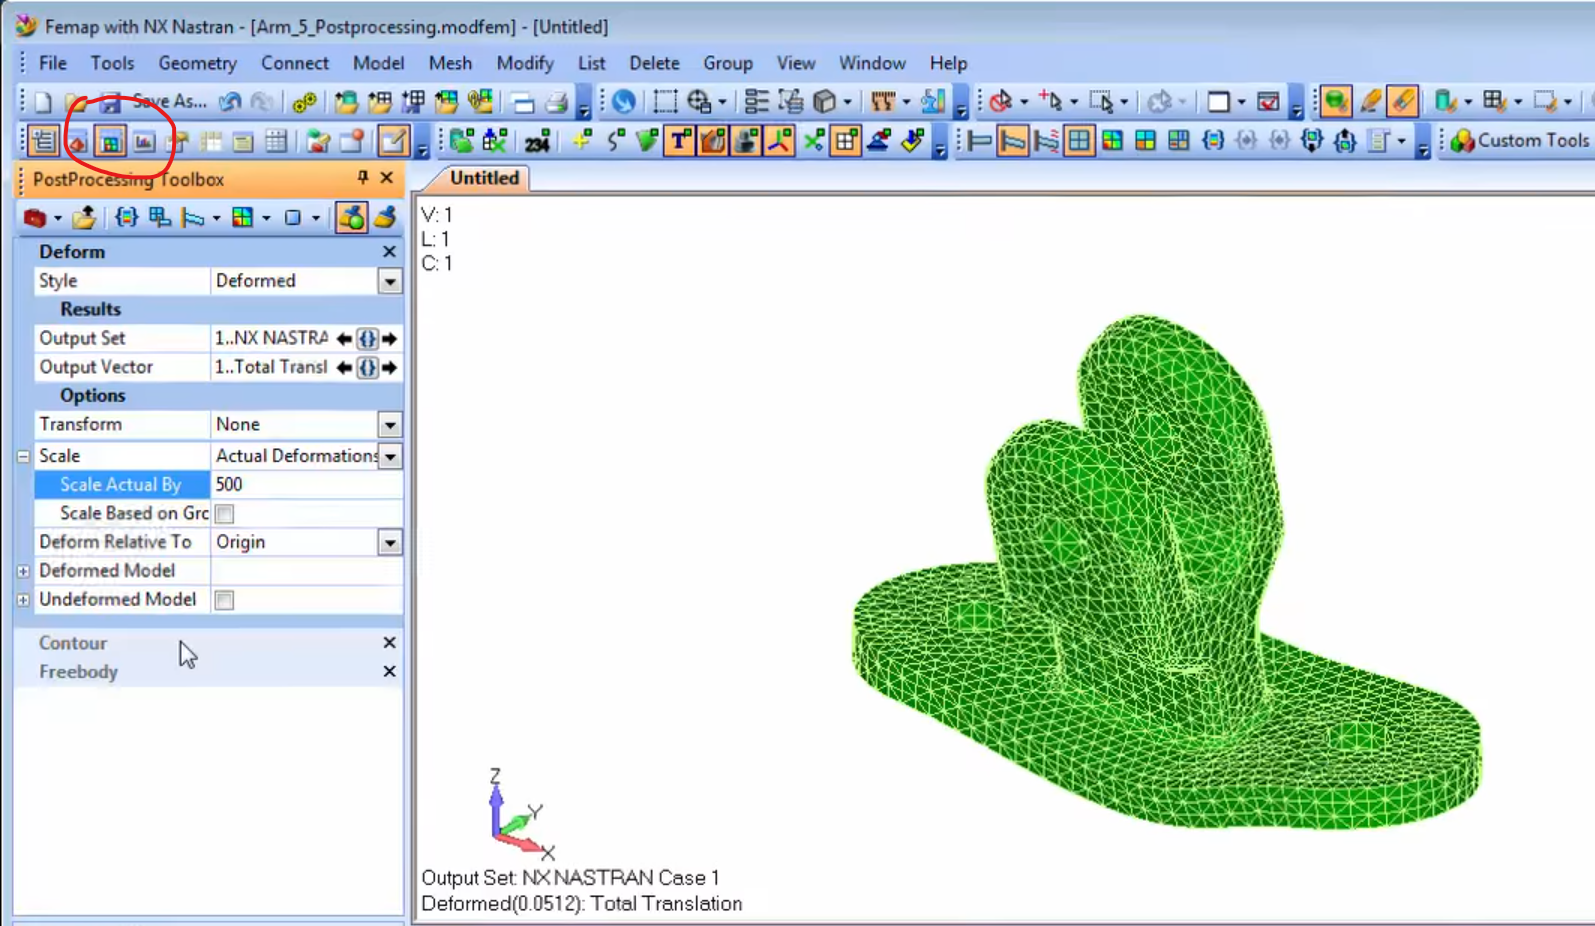
\includegraphics[width=12cm]{Femap13}
\caption{\Large Femap Deformed}\label{3.13}
\end{center}
\end{figure}
\\
\begin{figure}[hbt!]
\begin{center}
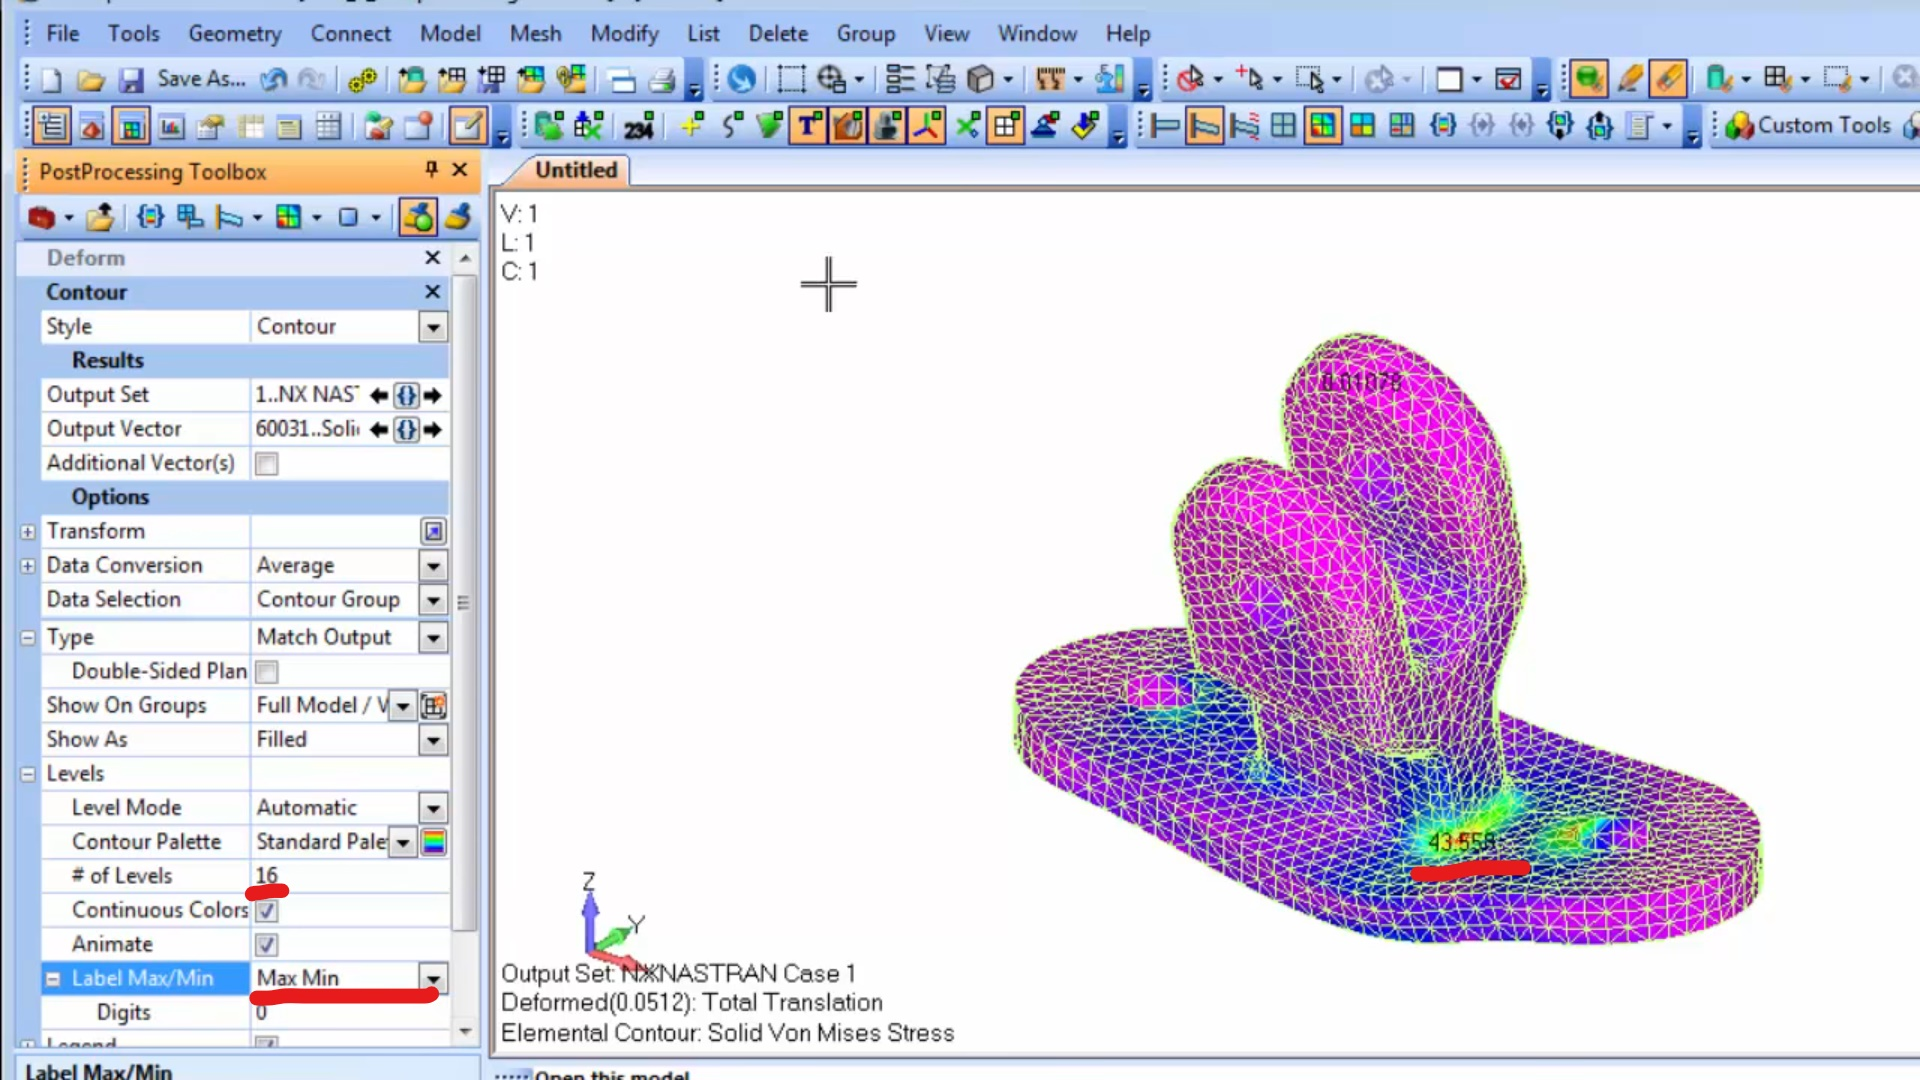
\includegraphics[width=12cm]{Femap14}
\caption{\Large Femap Contour}\label{3.14}
\end{center}
\end{figure}
\\
\begin{figure}[hbt!]
\begin{center}
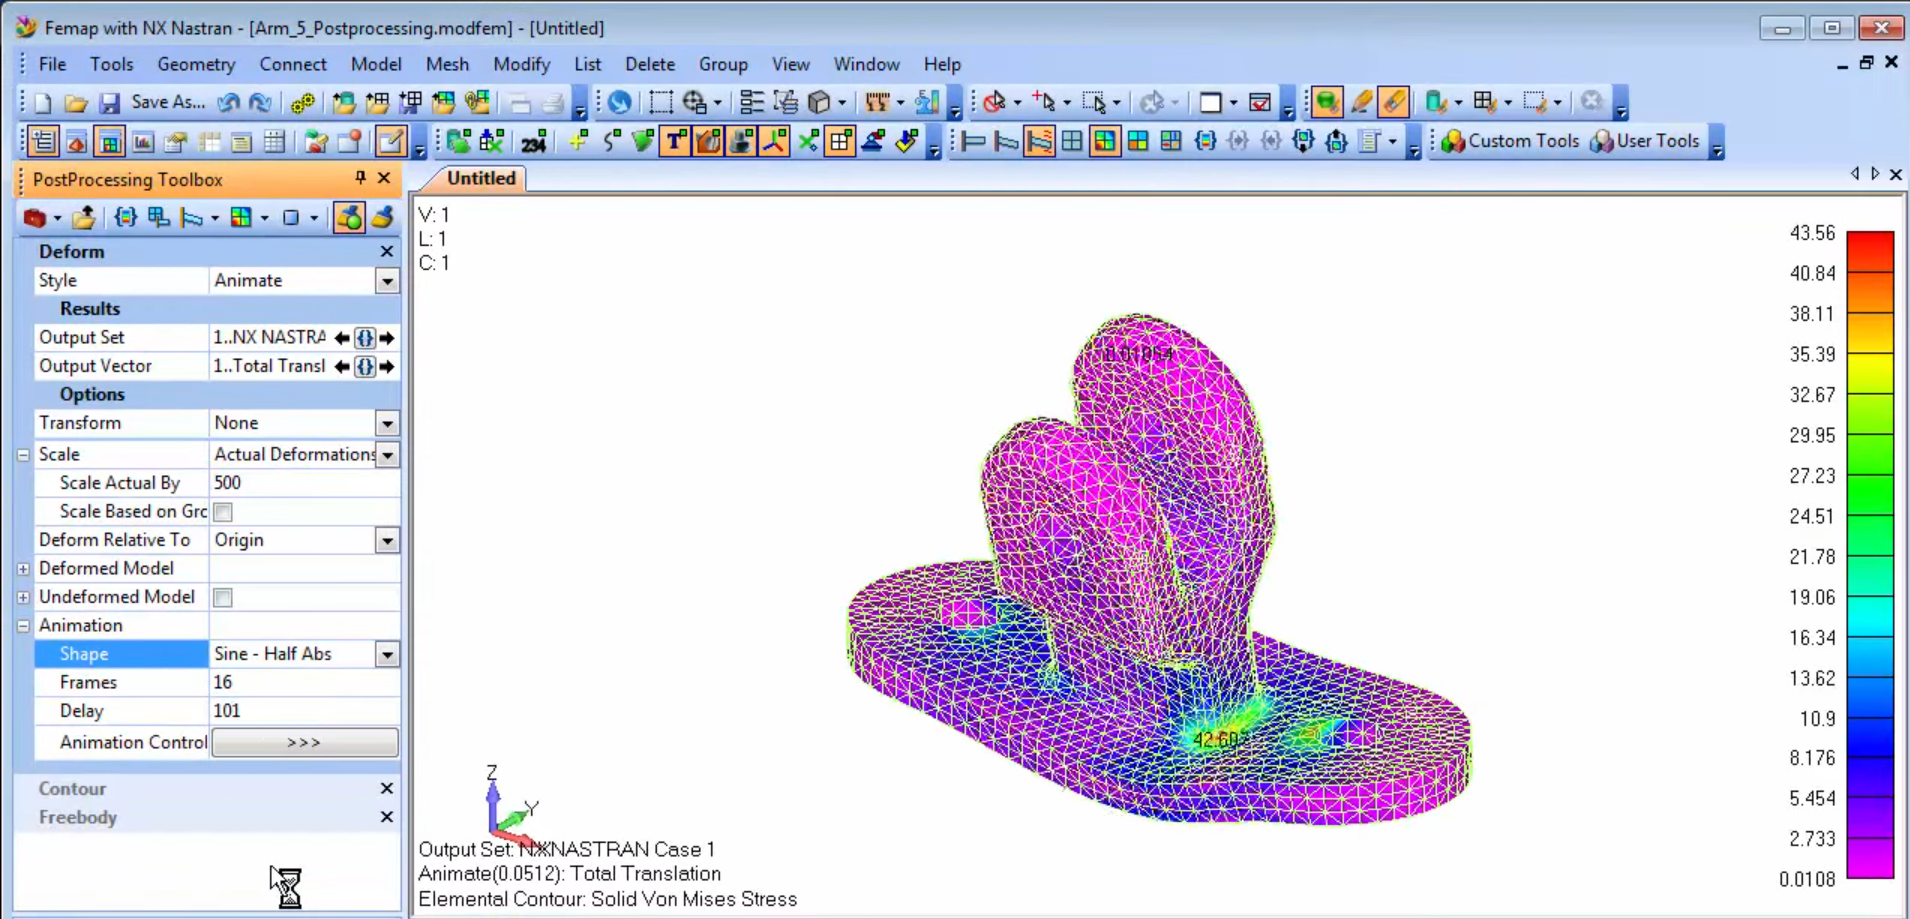
\includegraphics[width=12cm]{Femap15}
\caption{\Large Femap Animate}\label{3.15}
\end{center}
\end{figure}
\\
\end{itemize}

\section{Solid Edge與Femap在生成式機械設計上的應用範例}
















\newpage